\documentclass[../report.tex]{subfiles}

\begin{document}

\chapter{Literature Review}

This section contains review of papers in bibliography. From these we take the foundation \& implement it for one example.

\section{Lagrangian Approach}
Consider the Dynamical System,
\begin{equation}
  \begin{aligned}
    \frac{d}{dt}(x(t)) &= V(x(t), t) \\
    x_0 &= x(t_0) \\
    x \in \mathbb{R}^n &, t \in \mathbb{R}
  \end{aligned}
\end{equation}

For LCS, it is needed to compute Finite-Time-Lyapunov-Exponent (FTLE), with a FTLE for each grid point the structures can be plotted. \par

FTLE is a scaler \(\sigma_{t_0}^T(n)\) which represents structures of a fluid at a location. The maxima show the attracting (or repelling barriers). Let's say a particle at \(x(t_0)\) goes to a new location after time \(T\). \par

Flow map of that point can be written as
\begin{equation}
  F_{t_0}^t(x_0) = x_0 + \int_{t_0}^{T} V(x(t), t)\,dt
\end{equation}

Let's say there is another point close to \(x(t_0)\) which is \(y = x + \delta x(t_0)\). After a time interval \(T\), distance between these 2 points becomes
\begin{equation}
  \begin{aligned}
    \delta x(t_0 + T) &= F_{t_0}^{t_0 + T} (y) - F_{t_0}^{t_0 + T} (x) \\
    &= \nabla F_{t_0}^{t_0 + T}(x)
  \end{aligned}
\end{equation}

From above equation we can calculate the neon strain tensor,
\begin{equation}
  \begin{aligned}
    C &= \nabla {F_{t_0}^{t_0 + T}(x)}^T \cdot \nabla F_{t_0}^{t_0 + T}(n)
  \end{aligned}
\end{equation}

Eigan values of which are \(\lambda_1, \lambda_2, \dots, \lambda_n\) \& associated normalized eigenvectors, \(\epsilon_{\lambda_i}\;\; (i \in \{1, 2, 3, \dots, n\})\)

\(\therefore\) From the maximum eigenvalue of chuchy green tensor FTLE can be calculated as
\begin{equation}
  \begin{aligned}
    \sigma_{t_0}^T (x_0) = \frac{1}{2|T|} \log(\lambda_n)
  \end{aligned}
\end{equation}

\begin{equation}
  \begin{aligned}
    \lambda_n &= max\; eig (C) \\
    &= max\; eig(\nabla {F_{t_0}^{t_0 + T}(x)}^T \cdot \nabla F_{t_0}^{t_0 + T}(n))
  \end{aligned}
\end{equation}

To complete FTLE, it is necessary to have locations of particles at initial state \(t = t_0\) \& at \(t = t_0 + T\). \(\therefore\) Flow map can be determined.

\#TODO: Increase font size

\begin{equation}
  \begin{aligned}
    {F_{t_0}^{t_0 + T}} &= \begin{bmatrix}
      \frac{x_{i + 1, j}(t_0 + T) - x_{i - 1, j}(t_0 + T)}{x_{i+1, j}(t_0) - x_{i-1, j}(t_0)} & \frac{x_{i, j+1}(t_0 + T) - x_{i,j-1}(t_0 + T)}{y_{i,j+1}(t_0) - y_{i,j-1}(t_0)} \\[12pt]
      
      \frac{y_{i+1, j}(t_0 + T) - y_{i-1, j}(t_0 + T)}{x_{i+1,j}(t_0) - x_{i-1, j}(t_0)} & \frac{y_{i,j+1}(t_0 + T) - y_{i, j - 1}(t_0 + T)}{y_{i, j+1}(t_0) - y_{i, j-1}(t_0}
    \end{bmatrix}
  \end{aligned}
\end{equation}


~ \\ ~ \\
\begin{figure}[H]
  \centering
  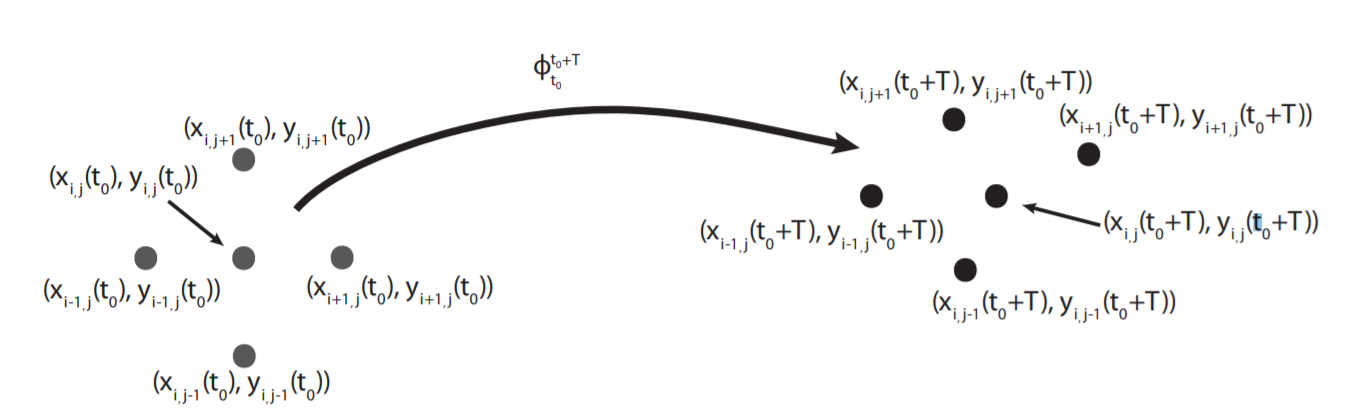
\includegraphics[width=0.8\linewidth]{images/image_1.png}
  \caption{Flowmap used for computing the FTLE}
  \label{fig:fig-1}
\end{figure}

Now let's see the Eulerian Approach. \par

\section{Eulerian Approach}
The Eulerian role of strain Tensor is defined as
\begin{equation}
  \begin{aligned}
    S(x, t) = \frac{1}{2}{\nabla V(x, t) + \nabla V(x, t)^T}
  \end{aligned}
\end{equation}
and eigan values of which are \(s_1 < s_2 < \dots < s_n\) and associated normalized eigen vectors, \(\epsilon_{S_i}\;\; i \in \{1, 2, \dots, n\}\) \par

From the eigen values of eulerian rate of stain tensor, one can identify regions of flow which are more attracting \& repelling. \par

There \(s_1\) \rightarrow minimum eigen values provides measure of attraction \& \(s_2\) maximum value of repulsion.

\subsection{Relation between Cauchy-Green Strain Tensor \& Eulerian Rate of Strain Tensor}
Eigen value of \(S\) as FTLE limit as integration of time goes to 0. \par

For small \(|T|\), let us expand  \(C_{t_0}^t (x)\) as
\begin{equation}
  \begin{aligned}
    C_{t_0}^t (n) &= 1 + 2T S(x, t_0) + T^2 B(x, t_0) + \frac{1}{2} T^3 Q(x, t_0) + O(T^4)
  \end{aligned}
\end{equation}

Where,
\begin{equation}
  \begin{aligned}
    B(x, t_0) &= \frac{1}{2}[\nabla a(x, t_0) + (\nabla a(x, t_0))^T] + \nabla V(x, t_0)^T \cdot \nabla V(x, t_0)
  \end{aligned}
\end{equation}

Where acceleration field \(a(x, t_0)\) is
\begin{equation}
  \begin{aligned}
    a(x, t_0) = \frac{d}{dt}V(x, t_0) = \frac{\partial}{\partial t} V(x, t_0) + V(x, t_0) \cdot \nabla V(x, t_0)
  \end{aligned}
\end{equation}

\begin{equation}
  \begin{aligned}
    \lambda_n &= \lambda^+ (C_{t_0}^t (x)) \text{for small, } T > 0
  \end{aligned}
\end{equation}

We can neglect \(O(T^2)\) in
\begin{equation}
  \begin{aligned}
    \therefore \lambda^+ (C_{t_0}^t (x)) &= 1 + 2T \lambda^+ (S(x, t_0)) + O(T^2)
  \end{aligned}
\end{equation}

\begin{equation}
  \begin{aligned}
    \log(\lambda_n) &= \log(1 + 2T\lambda^+S(x, t_0)) \\
    &= 2T\lambda^+(S(x, t_0)) \\
    &= 2Ts_n(x, t)
  \end{aligned}
\end{equation}

In the limit of small \(T,\; \log(1+\epsilon) = \epsilon\)

\begin{equation}
  \begin{aligned}
    \sigma_{t_0}^T &= \frac{1}{2|T|}\log(\lambda_n) \\
    &= \frac{1}{2T} \cdot 2T \cdot S(x, t_0) \\
    &= s_n(x, t_0)
  \end{aligned}
\end{equation}

For \(T < 0\), with small T
\begin{equation}
  \begin{aligned}
    \lambda^+ (C_{t_0}^t(x)) &= 1 + 2T \lambda^- (S(x, t_0))
  \end{aligned}
\end{equation}

\begin{equation}
  \begin{aligned}
    \log(\lambda_n) &= 2T\lambda^- (S(x, t_0)) \\
    &= 2Ts_1(x, t_0)
  \end{aligned}
\end{equation}

\(\therefore |T| = -T \text{if } T < 0\)
\begin{equation}
  \begin{aligned}
    \sigma_{t_0}^t &= \frac{1}{2|T|} \log(\lambda_n) = -s_1(x, t_0)
  \end{aligned}
\end{equation}

\(\therefore\) We can summarize as follows,
\begin{equation}
  \begin{aligned}
    \sigma_{t_0}^t &= \pm s^\pm (x, t_0)\; \text{as } t - t_0 \rightarrow 0^\pm
  \end{aligned}
\end{equation}

\begin{equation}
  \nabla V = \begin{bmatrix}
    \frac{\partial U}{\partial x} & \frac{\partial U}{\partial y} \\[12pt]
    \frac{\partial V}{\partial x} & \frac{\partial V}{\partial y} \\
  \end{bmatrix}
\end{equation}

\begin{equation}
  \nabla S = \begin{bmatrix}
    \frac{\partial U}{\partial x} & \frac{1}{2} (\frac{\partial U}{\partial y} + \frac{\partial V}{\partial x}) \\[12pt]
    \frac{1}{2} (\frac{\partial U}{\partial y} + \frac{\partial V}{\partial x}) & \frac{\partial V}{\partial y} \\
  \end{bmatrix}
\end{equation}

\subsection{Equality of Eigen Vectors of \(S\) \& \(C\)}
\begin{equation}
  \begin{aligned}
    S\epsilon_i &= S_i\epsilon_i \\
    2TS\epsilon_i + \epsilon_i &= 2TS_i\epsilon_i + \epsilon_i \\
    (2TS + 1)\epsilon_i &= (2TS_i + 1)\epsilon_i \\
    C\epsilon_i &= \lambda_i\epsilon_i
  \end{aligned}
\end{equation}

\(\Rightarrow \epsilon_i\) is an eigen vector of \(S\) then \(\epsilon_i\) is an eigen vector of \(C\).

\(\therefore\) We can say as \(T\) goes to 0, eigen vector of \(C\) is same as eigen vector of \(S\).

\end{document}